\documentclass[10pt,twocolumn]{article}
\usepackage{graphicx}
\usepackage{amssymb}
\usepackage{titling}
\usepackage{url,hyperref}

\begin{document}

\title{Predicting How New Yorkers Seek Medical Advice}

\author{Michelle Ho and Shay Lehmann}

\date{%
CUSP-GX-5006\\
Machine Learning Assignment \# 2\\
\rule{\textwidth}{1pt}
}

\posttitle{\par\rule{3in}{0.4pt}\end{center}\vskip 0.5em}
%\postdate{\rule{\textwidth}{1pt}}

\maketitle

\begin{abstract}
In this assignment, the authors explore how New Yorkers seek medical advice and how
this can be predicted by other variables found in the NYC Community Health Survey.
The exercise demonstrates that the use of Naive-Bayes and Support Vector Machine (SVM)
classification techniques and their in performance in a real life scenario.
\end{abstract}

\section{Introduction}
The main goal of this assignment is to demonstrate the use of two classification
techniques, Naive-Bayes and Support Vector Machine (SVM), on predicting how
New Yorkers seek medical advice.

The authors examined the results of the Community Health Survey (CHS) conducted
by the New York City Department of Health and Mental Hygiene. This rich dataset
includes measurements on multiple aspects of health-- including access, nutrition,
demographic information, diet and exercise habits, medical history, and lifestyle
choices.

The motivation is to better understand how New Yorkers seek and receive advice
for their medical needs. Outreach programs hoping to improve access to health care
can make use of these results.

\section{Methods and Data Sets}

The raw dataset of the 2014 NYC Community Health Survey contains 8562 observations
across 188 variables. For this assignment, a subset of the raw dataset was used
for analysis, and the variables are described below:

\begin{itemize}
\item Sick Advice: A categorical variable about the respondent's usual resource for
health advice. This is the dependent variable in the analyses for this
assignment. The options are
``A private doctor",
``Community health center",
``A hospital outpatient clinic",
``ED/urgent care center",
``Alternative health care provider",
``Family/friend/self/resources",
``Non-hospital clinic",
``Other",
``No usual place", or
``Clinic, unknown type".
\item Education: A categorical variable on educational attainment. Categories are ``Less than HS", ``High school grad",
``Some college", or ``College graduate"
\item Marital status: A categorical variable on marital status. Categories are
``Married",
``Divorced",
``Widowed",
``Separated",
``Never married", or
``Member of unmarried couple living together"
\item US born: A binary variable answering the yes or no question "Are you US or foreign born?"
\item Sexual ID: A categorical variable on sexual orientation. Categories are
``Heterosexual",
``Gay/Lesbian", or
``Bisexual"
\item At Home Language: A categorical variable answering the question ``What language do you
speak most often at
home?" Options are
``English",
``Spanish",
``Russian",
``Chinese",
``Indian", or
``Other"
\item Insured: A binary variable answering the yes or no question ``Do you have any
kind of health
insurance coverage,
including private
health insurance,
prepaid plans such as
H-M-Os, or
government plans
such as Medicare or
Medicaid?"
\item The dependent variable being classified and predicted is `Sick Advice' in this assignment's
analyses. The authors refer to this variable as `Y'. The goal is to attempt to
predict how people will seek their medical advice based on other characteristics.
\item The independent variables are all the others.
\item  For all variables, the options ``do not know" and ``refuse"
are treated as null values and dropped. After these drops, the number of observations
in the dataset is 7827.
\item Finally, independent variables are binarized so that all samples are represented
by boolean feature vectors.
\end{itemize}


The steps taken for this assignment:

\begin{enumerate}
\item A classification model is fitted for the binarized 6 independent variables with
a Naive Bayes algorithm assuming Bernoulli distributions.
\item A second classification model is fitted on the same variables with
a SVM using a linear kernel.
\item Finally, a third classification model is fitted with a SVM using a radial basis
function (RBF) kernel.
\item The authors adjust the RBF kernel parameters to assess how these parameters
affects the overall performance of the classification model and possible overfitting.
\item All models are assessed via cross validation on training and test sets split
from the original dataset. The training and test set sizes are adjusted to assess the effect of training size on quality
of classification.
\item The results of classification are visualized by projecting the observations
into their first two principle components and colored according to classification (Figure 1 - 2)
\item Confusion matrices are created for all categories of the dependent variable
``Sick Advice" to assess the performance of the classifications (Figure 3 - 4)
\end{enumerate}

\section{Results}

For our sample and variables, each model was run with training samples of 1550,
3101, 4652 and 6203, representing 20\%, 40\%, 60\% and 80\% of the data respectively.
The mean errors of in-sample and out-of-sample misclassifications for the 80-20 training-test
split for all models is reported in Table 1 at the end of this report.

The Naive Bayes model generally performed least well, with model trained on the
20\% of the data misclassifying 34.3488\%, the model trained on 40\% of the data
misclassifying 33.3333\% of the data, the model trained on 60\% of the data
misclassifying 34.4294\% of the data and the model trained on 80\% of the data
misclassifying 33.9136\% of the data. As a baseline, the mean
in-sample misclassification of the training sets with the generated Naive Bayes models
 was 31.3043\%.

The Linear SVM, on the other hand, sorted
every item into the Private Doctor category. However, in our dataset, this response had been
chosen by nearly 69\% of applicants so the SVM model actually performed better
than the Naive Bayes, misclassifying between 30.43\% of the data and 31.17\% of the data, depending
on training sample size. This aligns with how many people chose Private Doctor in the first place.
In other words, the Linear SVM model defaulted to the majority classification and yielded better
results than Naive Bayes.

We then ran SVM with an RBF kernel. This model misclassified a similar
percentage of test data points (30.75\% to 31.46\% depending on training size),
but placed people in more diverse
categories.

Lastly, the authors tried to give the 'hospital outpatient clinic', the second
most popular category, a weight of 3 using SVM with RBF kernel. However, this
performed even worse than the Naive Bayes, with misclassified data percentages of
35.11\%, 34.75\%, 35.59\% and 34.24\% for training sample sizes of 20\%, 40\%, 60\% and
80\% respectively.

\section{Conclusions}

In summary, the classification models performed poorly in predicting
how people tend to seek out medical advice based on other characteristics. This
may be because an overwhelming percentage of respondents chose private doctor so
the model actually performed best when sorting all people into that one category.
The authors' models were not able to improve upon this base model and only the
SVM with RBF kernel was able to match it while correctly identifying some of the
people in other categories.

Further steps for this assignment would include earlier years of data from the
NYC Community Health Survey to expand the dataset, since we have seen that training
size of the dataset can have an affect on classification models.

Python code used to generate the results, tables, and figures for this assignment can be
found at \url{https://github.com/michellemho/machine_learning_for_cities}.

\begin{center}
\begin{table*}[]
\centering
\caption{Classification Models (80-20 Split) Error (percentage)}
\label{my-label}
\begin{tabular}{lllll}
                & In-Sample Misclassification & Out-Sample Misclassification & \\
Naive Bayes        & 31.30              & 33.91                  & \\
SVM Linear    & 29.50              & 31.17               & \\
SVM RBF      & 30.01               & 31.46                & \\
SVM RBF classweight       & 34.50               & 34.24                  & \\
                &                           &                         &
\end{tabular}
\end{table*}
\end{center}

\begin{figure*}[!t]
  \begin{center}
    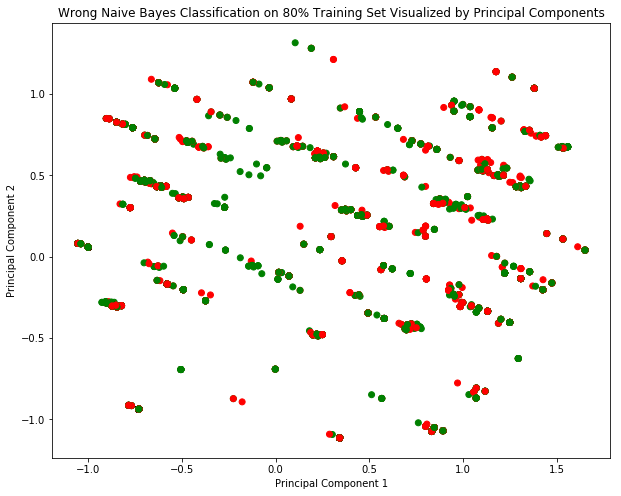
\includegraphics[width=6in]{pca.png}
  \end{center}

  \caption{\small The raw dataset visualized by PCA}
  \label{fig-1}
\end{figure*}

\begin{figure*}[!t]
  \begin{center}
    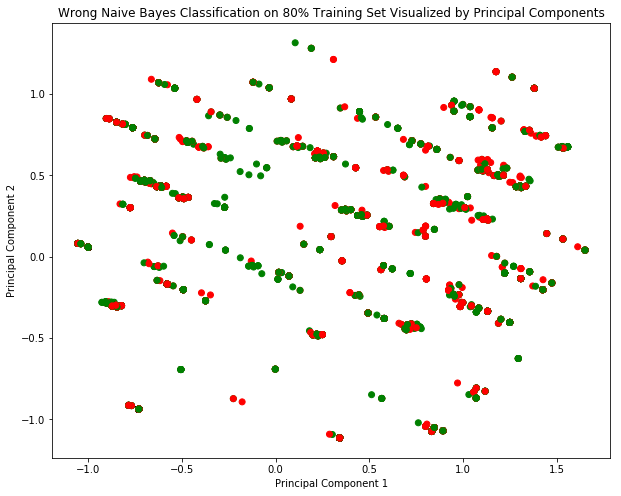
\includegraphics[width=6in]{pca.png}
  \end{center}

  \caption{\small The results of Naive Bayes Classifier}
  \label{fig-1}
\end{figure*}

\begin{figure*}[!t]
  \begin{center}
    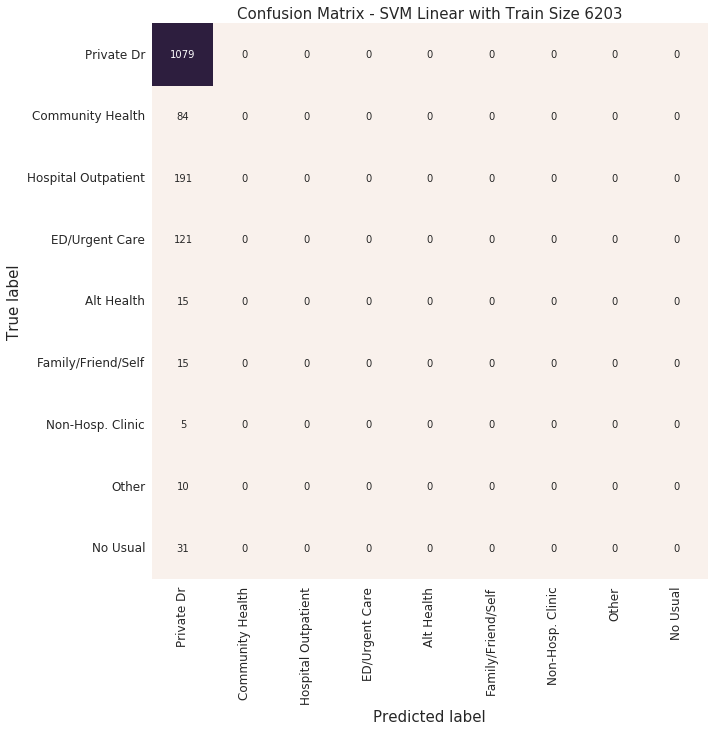
\includegraphics[width=6in]{confusion_matrix_SVM_Linear_6203.png}
  \end{center}

  \caption{\small Confusion Matrix showing the results of SVM with the Linear Kernel and
  80\% of the data including within the training sample. The diagonal is colored according to
  the percentage of True Positives. Note that all test data points were classified
  as 'Private Doctor'}
  \label{fig-2}
\end{figure*}

\begin{figure*}[!t]
  \begin{center}
    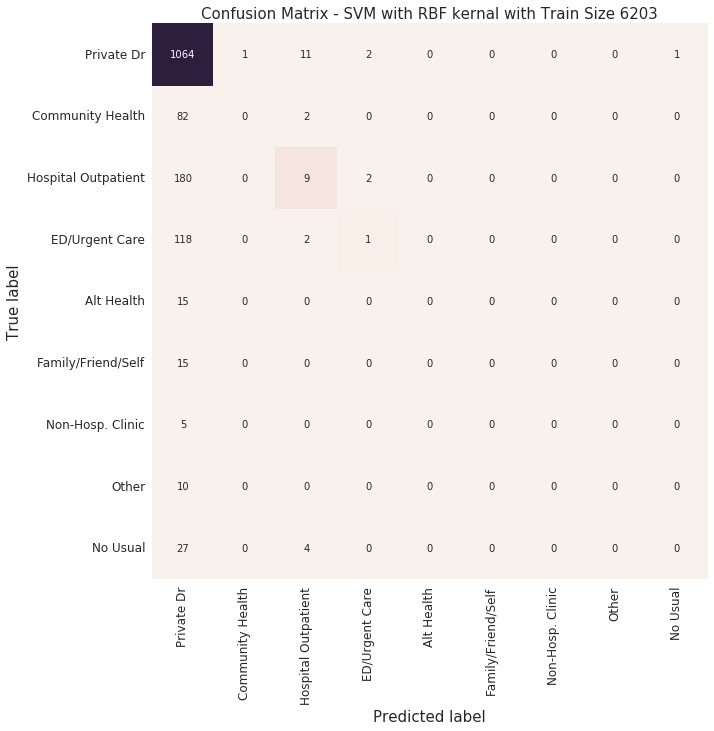
\includegraphics[width=6in]{confusion_matrix_RBF_CW1_6203.png}
  \end{center}

  \caption{\small Confusion Matrix showing the results of SVM with the RBF Kernel and
  80\% of the data including within the training sample. The diagonal is colored according to
  the percentage of True Positives}
  \label{fig-3}
\end{figure*}





\end{document}
